%%%%%%%%%%%%%%%%%%%%%%%%%%%%%%%%%%%%%%%%%%  不使用 authblk 包制作标题  %%%%%%%%%%%%%%%%%%%%%%%%%%%%%%%%%%%%%%%%%%%%%%
%-------------------------------PPT Title-------------------------------------
\title{12 多重散射与\rm{MTO}方法}
%-----------------------------------------------------------------------------

%----------------------------Author & Date------------------------------------
%\author[\textrm{Jun\_Jiang}]{姜\;\;骏\inst{}} %[]{} (optional, use only with lots of authors)
%% - Give the names in the same order as the appear in the paper.
%% - Use the \inst{?} command only if the authors have different
%%   affiliation.
%\institute[BCC]{\inst{}%
\institute[Gain~Strong]{\inst{}%
%\vskip -20pt 北京市计算中心}
\vskip -20pt {\large 格致斯创~科技}}
\date[\today] % (optional, should be abbreviation of conference name)
{%	{\fontsize{6.2pt}{4.2pt}\selectfont{\textcolor{blue}{E-mail:~}\url{jiangjun@bcc.ac.cn}}}
\vskip 45 pt {\fontsize{8.2pt}{6.2pt}\selectfont{%清华大学\;\;物理系% 报告地点
	\vskip 5 pt \textrm{2023.01.07}}}
}

%% - Either use conference name or its abbreviation
%% - Not really information to the audience, more for people (including
%%   yourself) who are reading the slides onlin%%   yourself) who are reading the slides onlin%%   yourself) who are reading the slides onlineee
%%%%%%%%%%%%%%%%%%%%%%%%%%%%%%%%%%%%%%%%%%%%%%%%%%%%%%%%%%%%%%%%%%%%%%%%%%%%%%%%%%%%%%%%%%%%%%%%%%%%%%%%%%%%%%%%%%%%%

\subject{}
% This is only inserted into the PDF information catalog. Can be left
% out.
%\maketitle
\frame
{
%	\frametitle{\fontsize{9.5pt}{5.2pt}\selectfont{\textcolor{orange}{“高通量并发式材料计算算法与软件”年度检查}}}
\titlepage
}
%-----------------------------------------------------------------------------

%------------------------------------------------------------------------------列出全文 outline ---------------------------------------------------------------------------------
%\section*{}
%\frame[allowframebreaks]
%{
%  \frametitle{Outline}
%%  \frametitle{\textcolor{mycolor}{\secname}}
%  \tableofcontents%[current,currentsection,currentsubsection]
%}
%%在每个section之前列出全部Outline
%%类似的在每个subsection之前列出全部Outline是\AtBeginSubsection[]
%\AtBeginSection[]
%{
%  \frame<handout:0>%[allowframebreaks]
%  {
%    \frametitle{Outline}
%%全部Outline中,本部分加亮
%    \tableofcontents[current,currentsection]
%  }
%}

%-----------------------------------------------PPT main Body------------------------------------------------------------------------------------
\small
%\section{\rm{VASP~}软件中\rm{PAW~}计算的实现}
%\frame
%
%	\frametitle{\textrm{VASP}计算的特色}
%	相比于与普通的第一原理计算软件,\textrm{VASP}很好地平衡了计算效率和精度的问题,总的来说,\textrm{VASP}主要通过这几个特色保证了计算的高效能
%	\begin{itemize}
%	     \item 迭代与优化算法的多样性\\
%		     本质上电荷密度迭代 \textrm{\&\&} 体系总能量优化是相同的优化问题,采用了类似的算法\upcite{CMS6-15_1996,PRB54-11169_1996}:\\
%			\textcolor{blue}{\textrm{Pseudo-Newton、Conjugate-Gradient、Broyden~mix、damping-factor、RMM-DIIS}}
%	     \item 尽可能采用局域基(原子轨道基)函数:~\\
%		     \textcolor{blue}{\textrm{LREAL}}=\textcolor{red}{\textrm{.TRUE.}}\\
%			优化的投影函数也尽可能在实空间表示
%	     \item \textrm{PAW}原子数据集:\textcolor{blue}{优异的赝势}\upcite{PRB59-1758_1999}
%	\end{itemize}
%}
\frame
{
	\frametitle{多重散射理论}
\begin{figure}[h!]
	\vspace{-5pt}
\centering
\animategraphics[autoplay, loop, height=1.2in]{1}{Figures/Multi_scattering-}{0}{9}
\label{Multiple_scattering}
\end{figure}
}

\section{\rm{MTO~}与\rm{LMTO~}方法}
\frame
{
\frametitle{\textrm{MTO}方法}
\textrm{MTO (Muffin-tin Orbial)}方法是\textrm{Andersen}于\textrm{1971}年提出的局域缀加基函数方案\upcite{Andersen_Book}。
%\textrm{MTO}的
\textcolor{blue}{目的:~用最小基组方法解析电子结构}

\textrm{MTO}的特点
\begin{itemize}
	\item \textcolor{red}{物理图像}:~和\textrm{APW}方法类似,要求基函数在\textrm{MT}球内、外分区域表示,并且在球面上连续
	\item \textcolor{red}{数学形式}:~基函数是最小优化基组
		\begin{enumerate}
			\item \textrm{MT}球内基函数是\textrm{MT}球的散射分波 
				$$\psi_l(\varepsilon,\vec r)=\mathrm{i}^lr^{-1}\phi_l(\varepsilon,\vec r)Y_L(\hat{\vec r})$$
		%	\item \textrm{MT}根据散射理论,\textrm{MT}球外基函数形如$$\psi_l(\varepsilon,\vec r)\propto j_l(q_0r)-\tan(\eta_l(\varepsilon))n_l(q_0r)$$
			\item 根据散射理论,\textrm{MT}球外波函数渐近行为近似是\textcolor{purple}{平面波叠加球面波},球面波用\textrm{Neumann~}函数展开,渐近波函数表示为$\psi_l(\varepsilon,\vec r)\propto j_l(q_0r)-\tan(\eta_l(\varepsilon))n_l(q_0r)$
		%	\item 当$\varepsilon<0$,\textrm{Neumann}函数$n_l$可用\textrm{Hankel}函数$h_l=j_l+\mathrm{i}\eta_l$替换,由此\textrm{MT}球外基函数形式为$$\psi_l(\varepsilon,\vec r)\propto\mathrm{i}^{-l}\mathrm{e}^{-|q_0|r}/|q_0|r$$
			\item 鉴于\textrm{Bessel~}函数会发散,当$\varepsilon<0$,\textrm{Neumann}函数$n_l$用\textrm{Hankel}函数$h_l=j_l+\mathrm{i}n_l$替换,确保正确的渐近行为\\
				\textcolor{red}{只有$\varepsilon$对应体系本征值时,函数在\textrm{MT}球面上连续}
		\end{enumerate}
\end{itemize}

%		特别地,当能量$\varepsilon<0$,\textrm{Neumannn}函数$n_l$用\textrm{Hankel}函数$h_l$代替$$h_l^{(1)}=j_l+\mathrm{i}\eta_l$$渐近形式为$\frac{\mathrm{i}^{-l}\mathrm{e}^{-|q_0|r}}{|q_0|r}$\\
%		此时球\textrm{Bessel}是非约束的,这样的轨道不适合做基函数:~因为当能量$\varepsilon<0$,只有当能量$\varepsilon=\varepsilon_{\vec k}$,球\textrm{Bessel}函数的系数为0,基函数才可能是正交归一
}

\frame
{
\frametitle{\textrm{MTO}方法的基函数}
%\textcolor{red}{“展开定理”可用来判断具有解析形式的函数是否适宜作为基函数:~}
%以$R$为中心的函数用临近位置的基函数展开
%\begin{displaymath}
%	\chi_{\alpha}(\vec r-\vec R)=\sum_{\alpha^{\prime}}B_{\alpha\alpha^{\prime}}(\vec R,\vec R^{\prime})\chi_{\alpha^{\prime}}(r-R^{\prime})
%\end{displaymath}
%该定理对于积分非常有用:~
%
上述单重散射模型给出的\textrm{MTO}函数不适宜作为\textrm{MTO~}基函数,\textrm{Andersen~}根据多重散射理论重构了基函数
		\begin{displaymath}
			\hspace*{-10pt}\chi_L^{\mathrm{MTO}}(\varepsilon,q_0,\vec r)=\mathrm{i}^lY_L(\hat{\vec r})\left\{
			\begin{aligned}
				&\psi_l(\varepsilon,r)+q_0\cot(\eta_l(\varepsilon))j_l(q_0r)&\quad r\leqslant S\\
				&q_0n_l(q_0r)&\quad r>S
			\end{aligned}\right.
		\end{displaymath}
		\textrm{Andersen~}构造的\textrm{MTO}基函数的特点
		\begin{itemize}
			\item \textcolor{blue}{\textrm{MT}球外部分函数形式简单}
			\item \textcolor{red}{\textrm{MTO}内的函数包含来自其他散射函数的贡献($j_l$部分)}
		\end{itemize}
		根据多重散射理论,球面波函数延伸到\textrm{MT}球外部分,可用球\textrm{Bessel}函数展开表示
		\begin{displaymath}
			n_L(q_0,\vec r-\vec R)=4\pi\sum_{L^{\prime}L^{\prime\prime}}C_{L^{\prime}L^{\prime\prime}}^Ln_{L^{\prime\prime}}^{\ast}(q_0,\vec R-\vec R\,^{\prime})j_{L^{\prime}}(q_0,\vec r-\vec R\,^{\prime})
		\end{displaymath}
		其中$C_{L^{\prime}L^{\prime\prime}}^L$是\textrm{Gaunt}系数

%		只有当能量参数$\varepsilon$对应体系的本征值时,用\textrm{MTO}基函数展开的波函数对应于体系本征态

		这里参数(衰减常数)$q_0$由$q_0^2=\varepsilon-V_0$确定
}

\frame
{
	\frametitle{\textrm{MTO}方法的基函数}
\begin{figure}[h!]
\centering
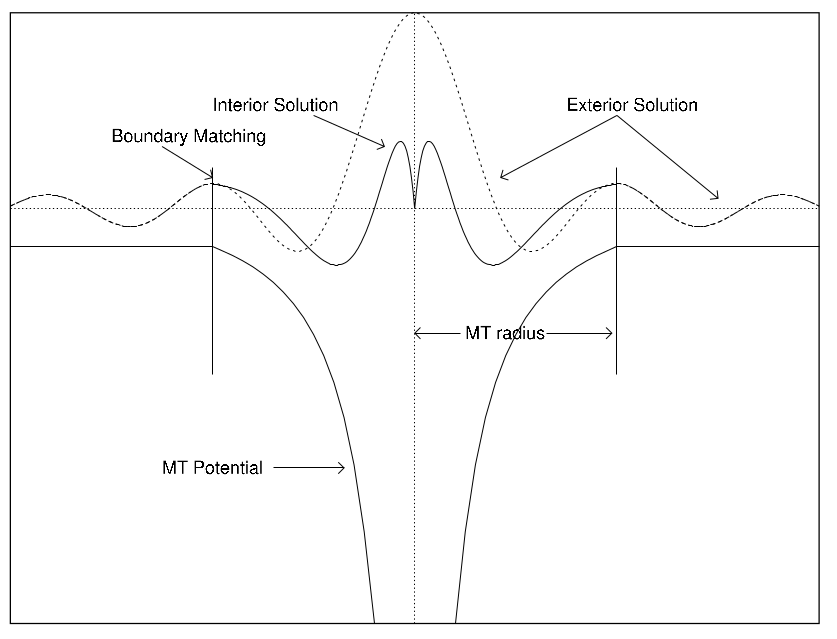
\includegraphics[height=1.55in,width=1.95in,viewport=0 0 845 635,clip]{Figures/MTO-envelope-1.png}
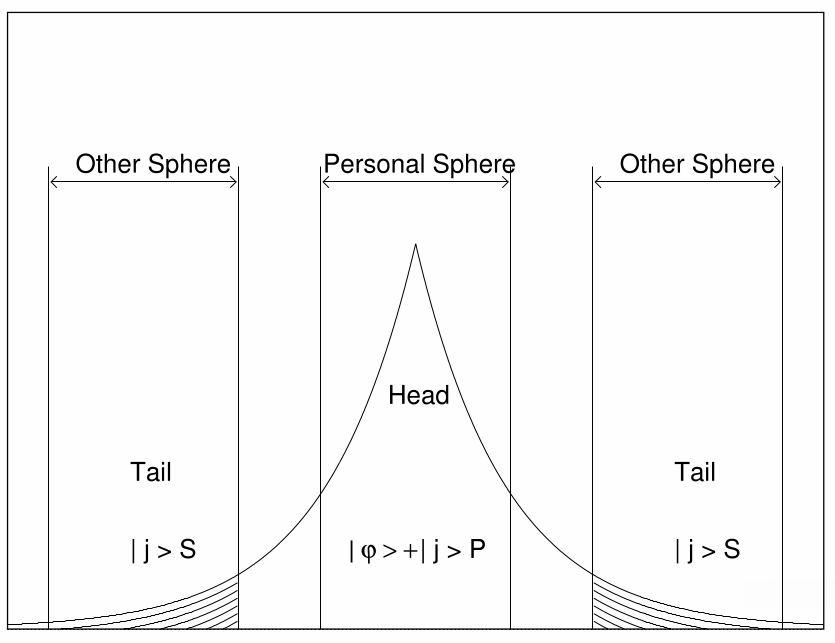
\includegraphics[height=1.55in,width=1.95in,viewport=0 0 885 635,clip]{Figures/MTO-envelope-2.png}
\caption{\tiny \textrm{The radial function of MTO expressed in different region.}}%(与文献\cite{EPJB33-47_2003}图1对比)
\label{MTO-envelope}
\end{figure}
}

\frame
{
	\frametitle{\textrm{MTO-ASA}}
\begin{figure}[h!]
	\vspace{-15pt}
\centering
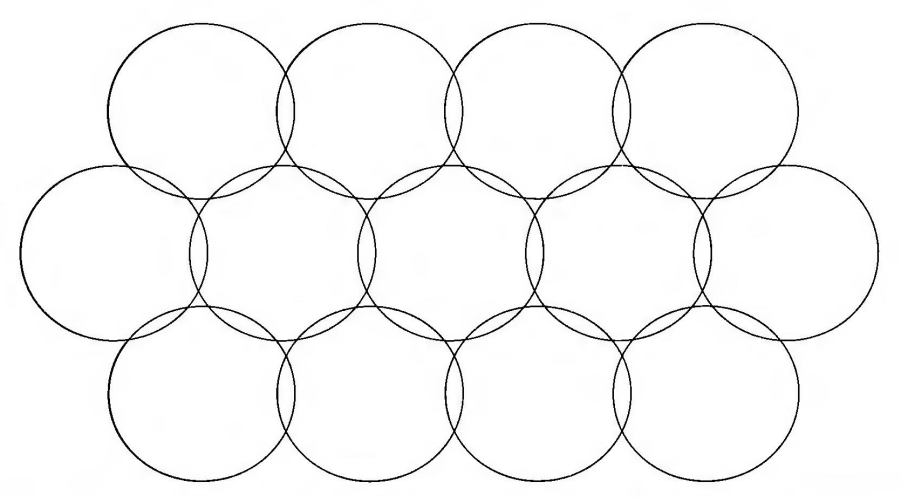
\includegraphics[height=1.20in,width=2.42in,viewport=5 0 1005 495,clip]{Figures/Atomic_sphere-appro.png}
\caption{\fontsize{8.2pt}{5.2pt}\selectfont\textrm{Atomic sphere approximation (ASA) in which the MT spheres are chosen to have the same volume as the Wigner-Seitz cell, which leads to overlapping spheres.}}

\label{Atomic_sphere-appro}
\end{figure}
当$q_0=0$时,构成最简单的\textrm{MTO}基函数
		\begin{displaymath}
			\hspace*{-12pt}\chi_L^{\mathrm{MTO}}(\varepsilon,0,\vec r)=\mathrm{i}^lY_L(\hat{\vec r})\psi_l(\varepsilon,S)\left\{
			\begin{aligned}
				&\dfrac{\psi_l(\varepsilon,r)}{\psi_l(\varepsilon,S)}-\dfrac{D_l(\varepsilon)+l+1}{2l+l}\left(\dfrac rS\right)^l&\, r\leqslant S\\
				&+\dfrac{l-D_l(\varepsilon)}{2l+1}\left(\dfrac Sr\right)^{l+1}&\, r>S
			\end{aligned}\right.
		\end{displaymath}
}

\frame
{
	\frametitle{正则能带基函数}
	$D_l(\varepsilon)$是径向分波$\psi_l(\varepsilon,r)$在球面$r=S$位置的对数导数
%	\begin{displaymath}
%		\hspace*{-15pt}\begin{aligned}
%			&\left[\dfrac S{|\vec r-\vec R|}\right]^{l+1}\mathrm{i}^lY_L(\widehat{\vec r-\vec R})\\
%				=&4\pi\sum_{L^{\prime}}\bigg[\dfrac rS\bigg]^{l^{\prime}}\mathrm{i}^{l^{\prime}}Y_{L^{\prime}}(\hat{\vec r})\left\{\dfrac{(2l^{\prime\prime}-1)!!}{(2l-1)!!(2l^{\prime}+1)!!}C_{L^{\prime}L^{\prime\prime}}^L\bigg[\dfrac S{|\vec R|}\bigg]^{l^{\prime\prime}+1}\mathrm{i}^{-l^{\prime\prime}}Y_{L^{\prime\prime}}^{\ast}(\hat{\vec R})\right\}
%		\end{aligned}
%	\end{displaymath}

	\textcolor{blue}{考虑平移周期性},
$$\chi_{L,\vec k}^{\mathrm{MTO}}(\varepsilon,0,\vec r)=\sum_{\vec T}\mathrm{e}^{\mathrm{i}\vec k\cdot\vec R}\chi_L^{\mathrm{MTO}}(\varepsilon,0,\vec r)$$
\textcolor{blue}{\textrm{MT}球内的\textrm{MTO-ASA}的基函数为}
{\fontsize{9.0pt}{5.2pt}\selectfont
\begin{displaymath}
	\begin{aligned}
		\chi_{L,\vec k}^{\mathrm{MTO}}(\varepsilon,0,\vec r)=&\underline{\textcolor{red}{\psi_l(\varepsilon,r)\mathrm{i}^lY_L(\hat{\vec r})}}-\dfrac{D_l(\varepsilon)+l+1}{2l+l}\psi_l(\varepsilon,S)\left(\dfrac rS\right)^l\mathrm{i}^lY_L(\hat{\vec r})\\
		&+\dfrac{l-D_l(\varepsilon)}{2l+1}\psi_l(\varepsilon,S)\sum_{L^{\prime}}\left(\dfrac rS\right)^{l^{\prime}}\dfrac1{2(2l^{\prime}+1)}\mathrm{i}^{l^{\prime}}Y_{L^{\prime}}(\hat{\vec r})S_{LL^{\prime}}(\vec k)
	\end{aligned}
\end{displaymath}}
其中
\begin{displaymath}
	\begin{aligned}
		S_{LL^{\prime}}(\vec k)=&2(2l+1)\dfrac{[D_l(\varepsilon)+l+1]}{[D_l(\varepsilon)-l]}\\
		=&g_{l^{\prime}m^{\prime},lm}\sum_{\vec T}\mathrm{e}^{\mathrm{i}\vec k\cdot\vec T}\bigg[\dfrac S{|\vec T|}\bigg]^{l^{\prime\prime}+1}\big[\sqrt{4\pi}\mathrm{i}^{l^{\prime\prime}}Y_{L^{\prime\prime}}(\hat{\vec T})\big]^{\ast}
	\end{aligned}
\end{displaymath}
}

\frame
{
	\frametitle{正则能带}
	\textcolor{red}{$\psi_l(\varepsilon,r)\mathrm{i}^lY_L(\hat{\vec r})$是\textrm{MT}球内满足原子分波函数的形式}
	\begin{itemize}
		\item \textcolor{blue}{在\textrm{MT}球内来自其他原子尾部贡献部分}$$\dfrac{l-D_l(\varepsilon)}{2l+1}\psi_l(\varepsilon,S)\sum_{L^{\prime}}\left(\dfrac rS\right)^{l^{\prime}}\dfrac1{2(2l^{\prime}+1)}\mathrm{i}^{l^{\prime}}Y_{L^{\prime}}(\hat{\vec r})S_{LL^{\prime}}(\vec k)$$
		\item \textcolor{blue}{在\textrm{MT}球内非物理贡献部分}$$\dfrac{D_l(\varepsilon)+l+1}{2l+l}\psi_l(\varepsilon,S)\left(\dfrac rS\right)^l\mathrm{i}^lY_L(\hat{\vec r})$$
	\end{itemize}
	\textcolor{red}{这两部分相互抵消},由此得到\textrm{MTO}中的\textrm{KKR}-型方程
	\begin{displaymath}
		\det[S_{LL^{\prime}}(\vec k)-P_l(\varepsilon)\delta_{LL^{\prime}}]=0
	\end{displaymath}
	这里$P_l(\varepsilon)$是“势函数”
	\begin{displaymath}
		P_l(\varepsilon)=2(2l+1)\dfrac{D_l(\varepsilon)+l+1}{D_{\varepsilon}-l}
	\end{displaymath}
	\textcolor{blue}{作变换$S_{LL^{\prime}}(\vec k)\xrightarrow{\bf{T}\rm{_u}}S_{lm,lm^{\prime}}(\vec k)$,由此确定的$\varepsilon_l(\vec k)$即正则能带}
}

\frame
{
	\frametitle{\textrm{MTO}轨道的“尾部抵消”}
\begin{figure}[h!]
	\vspace*{-0.7in}
\centering
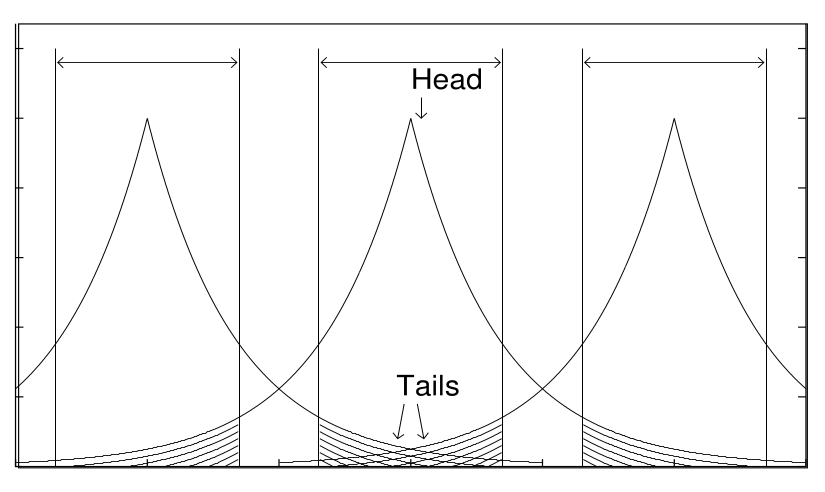
\includegraphics[height=2.55in,width=3.15in,viewport=0 0 845 635,clip]{Figures/MTO-Tail_cancellation.png}
\caption{\tiny \textrm{The wavefunction in the spere at the origin is the sum of the ``head function'' in that sphere plus the tails from neighboring spheres. The schematic illustration of the ``tail cancellation'' of the MTO.}}%(与文献\cite{EPJB33-47_2003}图1对比)
\label{MTO-tail-candellation}
\end{figure}
}

\frame
{
	\frametitle{\textrm{LMTO}方法}
	与\textrm{LAPW}方法类似,在给定能量$\varepsilon_v$和衰减常数$q_0$附近,\textrm{LMTO}的基函数球内部分用函数$\psi(\varepsilon_v,r)$及其对能量导数$\dot\psi(\varepsilon_v,r)$表示\\
\textcolor{blue}{\textrm{LMTO}与\textrm{MTO}基函数的区别}
	\begin{itemize}
		\item 球内部分的$\psi(\varepsilon,r)$是主要部分:~由$\psi(\varepsilon_v,r)$和$\dot\psi(\varepsilon_v,r)$线性组合
		\item 球内来自其它\textrm{MT}球的函数尾部贡献被$\dot\psi(\varepsilon_v,r)$的线性组合替代
	\end{itemize}
	由此根据物理直觉,可以把\textrm{LMTO}基函数的形式表示成
		\begin{displaymath}
			\hspace*{-12pt}\chi_L^{\mathrm{LMTO}}(\varepsilon,q_0,\vec r)=\mathrm{i}^lY_L(\hat{\vec r})\left\{
			\begin{aligned}
				&\psi_l(\varepsilon,r)-q_0\cot(\eta_l(\varepsilon))J_l(q_0r)&\, r\leqslant S\\
				&q_0N_l(q_0r)&\, r>S
			\end{aligned}\right.
		\end{displaymath}
		实际应用中,选定函数$J_l$和$N_l$与球\textrm{Bessel}函数$j_l$和\textrm{Neumann}函数$n_l$相似
}

\frame
{
	\frametitle{\textrm{LMTO}方法}
	根据物理边界要求,在\textrm{MT}球内,基函数$\chi_L^{\mathrm{LMTO}}$对能量$\varepsilon$的导数在$\varepsilon=\varepsilon_v$为0可确定$J_l$
		\begin{displaymath}
				J_l(q_0r)=-\dfrac{\dot\psi_l(\varepsilon_v,r)}{q_0\frac{\mathrm{d}}{\mathrm{d}\varepsilon}\cot(\eta_l(\varepsilon_v))},\,r\leqslant S
		\end{displaymath}
		$N_L$的定义与\textrm{Neumann}函数相似,在极限条件$n_l\rightarrow N_l$,$j_l\rightarrow J_l$,其它\textrm{MT}球的函数尾巴满足多重散射展开方式
		\begin{displaymath}
				N_L(q_0,\vec r-\vec R)=4\pi\sum_{L^{\prime},L^{\prime\prime}}C_{L^{\prime}L^{\prime\prime}}^Ln_{L^{\prime\prime}}^{\ast}(q_0,\vec R-\vec R\,^{\prime})J_{L^{\prime}}(q_0,\vec r-\vec R\,^{\prime}),\,r>S
		\end{displaymath}
		由此得到的能量无关的\textrm{LMTO}基函数满足
		\begin{itemize}
			\item \textcolor{blue}{在\textrm{MT}球内函数由$\psi$和$\dot\psi$的线性组合}
			\item \textcolor{blue}{\textrm{MT}球内函数光滑延伸到\textrm{MT}外,并能与其余\textrm{MT}球函数能量导数$\dot\psi$光滑连续}
		\end{itemize}
}

\frame
{
	\frametitle{\textrm{LMTO}方法}
	对于周期体系,取$q_0=0$~,\textrm{LMTO}方法的基函数可以表示为
	\begin{displaymath}
		\chi_{L,\vec k}^{\mathrm{LMTO}}(\vec r)=\dfrac{\psi_{l-}(\vec r)}{\psi_{l-}(S)}-\dfrac1{\psi_{l+}(S)}\sum_{L^{\prime}}\psi_{L^{\prime}+}(\vec r)\dfrac1{2(2l^{\prime}+1)}S_{LL^{\prime}}(\vec k)
	\end{displaymath}
	这里$\psi_{l-}(r)\equiv\psi_l(D=-l-1,r)$,$(r/S)^l\rightarrow\psi_{l+}(r)\equiv\psi_l(D=l,\varepsilon)$
	$$\psi(D,r)=\psi(r)+\omega(D)\dot\psi(r)$$
	这里
	$$\omega(D)=-\dfrac{\psi(S)D-D(\psi)}{\dot\psi(S)D-D(\dot\psi)}$$
	这里$D(\psi)$和$D(\dot\psi)$分别是$\psi$和$\dot\psi$的对数导数

	由此定义的\textrm{LMTO}基函数
	\begin{itemize}
		\item \textcolor{red}{对能量$\varepsilon_v$依赖到一阶}
		\item \textcolor{red}{径向函数在\textrm{MT}球外的尾巴抵消保持到计算所需要的最低阶}
	\end{itemize}
}

\frame
{
	\frametitle{固体计算方法总结}
\begin{figure}[h!]
\centering
\vspace*{-0.25in}
%\hspace*{-0.80in}
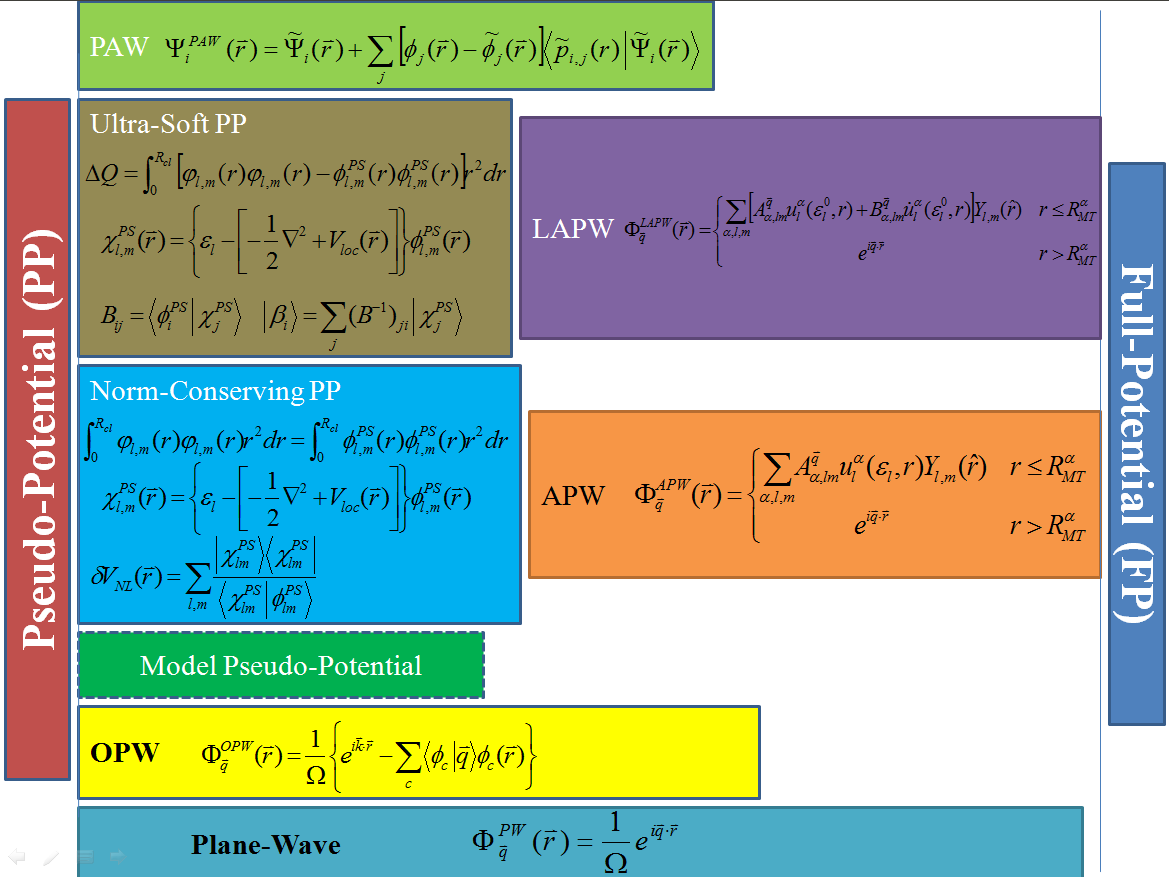
\includegraphics[height=2.80in,width=4.10in,viewport=0 0 1190 876,clip]{Figures/Pseudo-Full_Potential.png}
%\caption{\tiny \textrm{Pseudopotential for metallic sodium, based on the empty core model and screened by the Thomas-Fermi dielectric function.}}%(与文献\cite{EPJB33-47_2003}图1对比)
\label{Pseudo-Full_Poential}
\end{figure}
}

%------------------------------------------------------------------------Reference----------------------------------------------------------------------------------------------
		\frame[allowframebreaks]
{
\begin{thebibliography}{99}
\frametitle{主要参考文献}
{\tiny
	\bibitem{Singh}\textrm{D. J. Singh. \textit{Plane Wave, PseudoPotential and the LAPW method} (Kluwer Academic, Boston,USA, 1994)}
	\bibitem{Nemoshkalenko-Antonov}\textrm{V. V. Nemoshkalenko and V. N. Antonov. \textit{Computational Methods in Solid State Physics} (Gordon and Breach Science Publisher, Amsterdam, The Netherlands, 1998)}
	\bibitem{WIEN2k_UG}\textrm{P. Blaha, K. Schwarz, G. Madsen, D. Kvasnicka and J. Luitz. \textit{User's Guide of WIEN2K, An Augmented Plane Wave Plus Local Orbitals Program for Calculating Crystal Properties}. Vienna University of Technology, Inst. of Physical and Theoretical Chemistry, Vienna, Austria (2012)}
        \bibitem{PRB47-10142_1993}\textrm{K. Laasonen, A. Pasquarello, R. Car, C. Lee and D. Vanderbilt \textit{Phys. Rev.} B, \textbf{47} (1993), 10142}
	\bibitem{PRB12-3060_1975}\textrm{O. K. Andersen. \textit{Phys. Rev.} B, \textbf{12} (1971), 3060}
	\bibitem{JMP22-2433_1981}\textrm{M. Weiner. \textit{J. Math. Phys.}, \textbf{22} (1981), 2433}
	\bibitem{PRB26-4571_1982}\textrm{M. Weinert, E. Wimmer and A. J. Freeman. \textit{Phys. Rev.} B, \textbf{26} (1982), 4571}
	\bibitem{SSC114-15_2000}\textrm{E. Sj\"ostedt, L. Nordstr\"om and D. J. Singh. \textit{Solid State Commun.}, \textbf{114} (2000), 15}
	\bibitem{PR94-1111_1954}\textrm{W. Kohn and N. Rostocker. \textit{Phys. Rev.} \textbf{94} (1954), 1111}
	\bibitem{Andersen_Book}\textrm{O. K. Andersen. \textit{Computational Methods in Band Theory} (Plenum, New York, USA, 1971)}
	\bibitem{LMTO_Book}\textrm{H. Skriver. \textit{The LMTO method} (Springer, New York, USA, 1984)}
	\bibitem{JPCM14-2799_2002}\textrm{N. Papanikolaou, R. Zeller and P. H. Dederichs. \textit{J. Phys.: Condens. Matter.} \textbf{14} (2002), 2799}
}
\end{thebibliography}
\nocite*{}
}
%-----------------------------------------------------------------------------------------------------------------------------------------------------------------------%
